% Properly spaced highlight
\definecolor{light-gray}{gray}{0.85}
\setlength{\fboxsep}{0pt}%
\newcommand\reducedstrut{\vrule width 0pt height .9\ht\strutbox depth .4\dp\strutbox\relax}
\newcommand\hl[1]{\!\colorbox{light-gray}{\,\ensuremath{\reducedstrut#1}\,}}
\def\nquad{\hspace{-20pt}}

% Highlighted infrule/infax
\def\hlrule[#1]{\maybeindex{#1}\hlrulee{\inflabel{#1}}}
\def\hlrulee#1#2#3{\layoutrule{#1}{\colorbox{light-gray}{\ensuremath{\typesetrule{#2}{#3}}\ignorespaces}}}
\def\hlax[#1]{\maybeindex{#1}\hlaxx{\inflabel{#1}}}
\def\hlaxx#1#2{\layoutrule{#1}{\colorbox{light-gray}{\ensuremath{\reducedstrut{#2}}\ignorespaces}}}

\def\thirdA{\begin{minipage}[t]{0.32\linewidth}}
\def\thirdB{\end{minipage}\begin{minipage}[t]{0.32\linewidth}}
\def\thirdC{\end{minipage}\begin{minipage}[t]{0.32\linewidth}}
\def\thirdD{\end{minipage}\medskip\smallskip}
\def\halfA{\hspace{0.04\linewidth}\begin{minipage}[t]{0.45\linewidth}}
\def\halfB{\end{minipage}\hspace{0.02\linewidth}\begin{minipage}[t]{0.45\linewidth}}
\def\halfC{\end{minipage}\medskip\smallskip}

\newcommand\FMSyntaxEvaluation[1]{
  \begin{figure}%
  \begin{framed}%
  \begin{minipage}[t]{\linewidth}%
    \textit{Syntax}%
  \end{minipage}%

  \begin{minipage}[t]{.40\linewidth}%
    \vspace{-10pt}%
    \hfuzz=50pt
    \begin{flalign*}%
    \t \Coloneqq ~&&
      \\[-3pt] & \x                         & \textit{variable}
      \\[-3pt] & \λ\x \: \T.~ \t             & \textit{abstraction}
      \\[-3pt] & \λ\X \<: \T.~ \t            & \textit{type abstraction}
      \\[-3pt] & \t~\t                      & \textit{application}
      \\[-3pt] & \t~\T                      & \textit{type application}
      \\[-3pt] & \hl{\new \C}               & \textit{constructor call}
      \\[-3pt] & \hl{\t~\match \{ \overline{\x \: \C \⇒ \t} \} \otherwise~\t}
                                     \nquad & \textit{match expr.}
      \\
    \v \Coloneqq ~&&
      \\[-3pt] & \λ\x \: \T.~\t              & \textit{abstraction}
      \\[-3pt] & \λ\X \<: \T.~\t             & \textit{type abstraction}
      \\[-3pt] & \hl{\new \C}               & \textit{constructor call}
    \end{flalign*}%
    \hfuzz=0pt
  \end{minipage}%
  \hfill%
  \vline%
  \hfill%
  \begin{minipage}[t]{.40\linewidth}%
    \vspace{-10pt}%
    \hfuzz=50pt
    \begin{flalign*}%
    \T \Coloneqq ~&&
      \\[-3pt] & \X                         & \textit{type variable}
      \\[-3pt] & \T \rightarrow \T          & \textit{type of functions}
      \\[-3pt] & \forall \X \<: \T.~\T      & \textit{universal type}
      \\[-3pt] & \Top                       & \textit{maximum type}
      \\[-3pt] & \hl{\C}                    & \textit{class}
      \\[-3pt] & \hl{\{ \new \C \}} \nquad  & \textit{constructor singleton}
      \\[-3pt] & \hl{\T~\match \{ \overline{\T \⇒ \T} \} \otherwise~\T}
                                     \nquad & \textit{match type}
      \\
    \Γ \Coloneqq ~&&
      \\[-3pt] & \Ø                         & \textit{empty context}
      \\[-3pt] & \Γ, \x \: \T                & \textit{term binding}
      \\[-3pt] & \Γ, \X \<: \T               & \textit{type binding}
    \end{flalign*}%
    \hfuzz=0pt
  \end{minipage}%
  \end{framed}%
  \medskip
  \begin{framed}%
  \begin{minipage}[t]{\linewidth}%
    \textit{Evaluation}
    \medskip

    \thirdA
    \infrule[E-App1]
      { \t_1 \⟶ \t_1' }
      { \t_1~\t_2 \⟶ \t_1'~\t_2 }
    \thirdB
    \infrule[E-App2]
      { \t_2 \⟶ \t_2' }
      { \v_1~\t_2 \⟶ \v_1~\t_2' }
    \thirdC
    \infrule[E-TApp]
      { \t_1 \⟶ \t_1' }
      { \t_1~\T_2 \⟶ \t_1'~\T_2 }
    \thirdD

    \halfA
    \infax[E-AppAbs]
      { (\λ\x \: \T_{11}.~\t_{12})~\v_2 \⟶ [\x \↦ \v_2]\t_{12} }
    \halfB
    \infax[E-TAppTAbs]
      { (\λ\X \<: \T_{11}.~\t_{12})~\T_2 \⟶ [\X \↦ \T_2]\t_{12}}
    \halfC

    \begin{center}
    \begin{minipage}[T]{0.8\linewidth}
    \hlrule[E-Match1]
      { \t_s \⟶ \t'_s }
      { \,\t_s\match \{ \x_i \: \C_i \⇒ \t_i \} \otherwise~\t_d \⟶\\
         \t'_s\match \{ \x_i \: \C_i \⇒ \t_i \} \otherwise~\t_d \hphantom{\⟶}}
    \bigskip
    \hlrule[E-Match2]
      { (\C, \C_n) \∈ \Ψ  \andalso
        \∀m<n.~(\C, \C_m) \∉ \Ψ}
      { \new \C~\match \{ \x_i \: \C_i \⇒ \t_i\} \otherwise~\t_d \⟶ [\x_n \↦ \new \C]\t_n }
    \bigskip
    \hlrule[E-Match3]
      { \∀m.~(\C, \C_m) \∉ \Ψ }
      { \new \C~\match \{ \x_i \: \C_i \⇒ \t_i\} \otherwise~\t_d \⟶ \t_d }
    \bigskip
    \hlax[E-Match4]
      { \,(\λ\x \: \T.~\t)\match \{ \x_i \: \C_i \⇒ \t_i\} \otherwise~\t_d \⟶ \t_d\, }
    \bigskip
    \hlax[E-Match5]
      { \,(\λ\X \<: \T.~\t)\match \{ \x_i \: \C_i \⇒ \t_i\} \otherwise~\t_d \⟶ \t_d\, }
    \end{minipage}
    \end{center}
  \end{minipage}%
  \end{framed}%
  \caption{#1}%
  \label{fig:FMSyntaxEvaluation}%
  \end{figure}%
}

\newcommand\FMTypingRules[1]{
  \thispagestyle{empty}%
  \begin{figure}%
  \vspace{-20pt}%
  \begin{framed}%
  \begin{minipage}[t]{\linewidth}%
    \textit{Subtyping} %%%%%%%%%%%%%%%%%%%%%%%%%%%%%%%%%%%%%%%%%%%%%%%%%%%%

    \halfA
    \infax[S-Refl]
      { \Γ \⊢ \S \<: \S }
    \halfB
    \infax[S-Top]
      { \Γ \⊢ \S \<: \Top }
    \halfC

    \halfA
    \hlax[S-Sin]
      { \,\Γ \⊢ \{ \new \C \} \<: \C\, }
    \halfB
    \hlrule[S-Psi]
      { (\C_1, \C_2) \∈ \Ψ }
      { \Γ \⊢ \C_1 \<: \C_2 }
    \halfC

    \halfA
    \infrule[S-Trans]
      { \Γ \⊢ \S \<: \U  \andalso  \Γ \⊢ \U \<: \T }
      { \Γ \⊢ \S \<: \T }
    \halfB
    \infrule[S-Arrow]
      { \Γ \⊢ \T_1 \<: \S_1  \andalso  \Γ \⊢ \S_2 \<: \T_2 }
      { \Γ \⊢ \S_1 \→ \S_2 \<: \T_1 \→ \T_2 }
    \halfC

    \halfA
    \infrule[S-TVar]
      { \X \<: \T \∈ \Γ }
      { \Γ \⊢ \X \<: \T }
    \halfB
    \infrule[S-All]
      { \Γ, \X \<: \U_1 \⊢ \S_2 \<: \T_2 }
      { \Γ \⊢ (\∀\X \<: \U_1.~\S_2) \<: (\∀\X \<: \U_1.~\T_2) }
    \halfC

    \halfA
    \hlrule[S-Match1/2]
      { \Γ \⊢ \T_s \<: \S_n  \andalso  \∀m<n.~\Γ \⊢ \disj(\T_s, \S_m) }
      { \Γ \⊢ \T_s~\match \{ \S_i \⇒ \T_i \} \otherwise~\T_d \≡ \T_n }
    \halfB
    \hlrule[S-Match3/4]
      { \∀n.~\Γ \⊢ \disj(\T_s, \S_n) }
      { \Γ \⊢ \T_s~\match \{ \S_i \⇒ \T_i \} \otherwise~\T_d \≡ \T_d }
    \halfC

    \begin{center}
    \begin{minipage}[t]{.7\linewidth}
    \hlrule[S-Match5]
      { \Γ \⊢ \S_s \<: \T_s  \andalso  \Γ \⊢ \S_d \<: \T_d  \andalso  \∀n.~\Γ \⊢ \S_n \<: \T_n  }
      { \Γ \⊢ \S_s~\match \{ \U_i \⇒ \S_i \} \otherwise~\S_d \<: \\
         \hphantom{\Γ \⊢~} \T_s~\match \{ \U_i \⇒ \T_i \} \otherwise~\T_d \hphantom{\<:}}
    \end{minipage}
    \end{center}

    \vspace{5pt}
    \textit{Typing} %%%%%%%%%%%%%%%%%%%%%%%%%%%%%%%%%%%%%%%%%%%%%%%%%%%%%%%

    \halfA
    \infrule[T-Abs]
      { \Γ, \x \: \T_1 \⊢ \t_2 \: \T_2 }
      { \Γ \⊢ \λ\x \: \T_1.~\t_2 \: \T_1 \→ \T_2 }
    \halfB
    \infrule[T-App]
      { \Γ \⊢ \t_1 \: \T_{11} \→ \T_{12}  \andalso  \Γ \⊢ \t_2 \: \T_{11} }
      { \Γ \⊢ \t_1~\t_2 \: \T_{12} }
    \halfC

    \halfA
    \infrule[T-TAbs]
      { \Γ, \X \<: \U_1 \⊢ \t_2 \: \T_2  }
      { \Γ \⊢ \λ\X \<: \U_1.~\t_2 \: \∀\X \<: \U_1.~\T_2 }
    \halfB
    \infrule[T-TApp]
      { \Γ \⊢ \t_1 \: \∀\X \<: \T_{11}.~\T_{12}  \andalso  \Γ \⊢ \T_2 \<: \T_{11} }
      { \Γ \⊢ \t_1~\T_2 \:~[\X \↦ \T_2]\T_{12} }
    \halfC

    \begin{minipage}[t]{0.24\linewidth}
    \infrule[T-Var]
      { \x \: \T \∈ \Γ}
      { \Γ \⊢ \x \: \T }
    \end{minipage}
    \begin{minipage}[t]{0.36\linewidth}
    \infrule[T-Sub]
      { \Γ \⊢ \t \: \S  \andalso  \Γ \⊢ \S \<: \T }
      { \Γ \⊢ \t \: \T }
    \end{minipage}
    \begin{minipage}[t]{0.36\linewidth}
    \hlax[T-Class]
      { \,\Γ \⊢ \new \C \: \{ \new \C \}\, }
    \end{minipage}

    \begin{center}
    \begin{minipage}[t]{0.8\linewidth}
    \hlrule[T-Match]
      { \Γ \⊢ \t_s \: \T_s  \andalso  \Γ, \x_i \: \C_i \⊢ \t_i \: \T_i  \andalso  \Γ \⊢ \t_d \: \T_d}
      { \Γ \⊢ \t_s~\match \{ \x_i \: \C_i \⇒ \t_i \} \otherwise~\t_d \:
              \T_s~\match \{ \C_i \⇒ \T_i \} \otherwise~\T_d }
    \end{minipage}
    \end{center}

    \vspace{5pt}
    \textit{Disjointness} %%%%%%%%%%%%%%%%%%%%%%%%%%%%%%%%%%%%%%%%%%%%%%%%%

    \halfA
    \hlrule[D-Xi]
      { (\C_1, \C_2) \∈ \Ξ }
      { \Γ \⊢ \disj(\C_1, \C_2) }
    \halfB
    \hlrule[D-Psi]
      { (\C_1, \C_2) \∉ \Ψ }
      { \Γ \⊢ \disj(\{ \new \C_1 \}, \C_2) }
    \halfC

    \halfA
    \hlrule[D-Sub]
      { \Γ \⊢ \S \<: \U  \andalso  \Γ \⊢ \disj(\U, \T) }
      { \Γ \⊢ \disj(\S, \T) }
    \halfB
    \vspace{-15pt}
    \hlax[D-Arrow]
      { \,\Γ \⊢ \disj(\T_1 \→ \T_2, \C)\, }
    \vspace{7pt}
    \hlax[D-All]
      { \,\Γ \⊢ \disj(\∀\X \<: \T_1.~\T_2, \C)\, }
    \halfC
  \end{minipage}%
  \end{framed}%
  \caption{#1}%
  \vspace{-37.2pt}%
  \label{fig:FMTypingRules}%
  \end{figure}%
}

\newcommand\FMExtension[1]{
  \begin{figure}%
  \begin{framed}%
  \begin{minipage}[t]{\linewidth}%
    \begin{minipage}[t]{\linewidth}%
      \textit{Syntax}%
    \end{minipage}%

    \begin{minipage}[t]{.40\linewidth}%
      \vspace{-10pt}%
      \hfuzz=50pt
      \begin{flalign*}%
      \hl{\C \Coloneqq} ~&&
        \\[-3pt] & \hl{\A   } & \textit{ground class}
        \\[-3pt] & \hl{\B~\T} & \textit{parametric class}
        \\
      \end{flalign*}%
      \vspace{-28pt}%
    \end{minipage}%
    \hfill%
    \vline%
    \hfill%
    \begin{minipage}[t]{.40\linewidth}%
      \vspace{-10pt}%
      \hfuzz=50pt
      \begin{flalign*}%
      \t \Coloneqq \dots ~&&
        \\[-3pt] & \t~\match ~\hl{[\X]} \{ \overline{\x \: \C \⇒ \t} \} \otherwise~\t
                                       & \textit{match expr.}
        \\
      \T \Coloneqq \dots ~&&
        \\[-3pt] & \T~\match ~\hl{[\X]} \{ \overline{\T \⇒ \T} \} \otherwise~\T
                                       & \textit{match type}
        \\
      \end{flalign*}%
      \vspace{-28pt}%
    \end{minipage}%

    \textit{Evaluation} %%%%%%%%%%%%%%%%%%%%%%%%%%%%%%%%%%%%%%%%%%%%%%%%%%%
    \bigskip

    \infrule[BE-Match2]
      { (\C, \hl{[\X \↦ \U]} \C_n) \∈ \Ψ  \andalso
        \∀m<n.\,\hl{\∀\T.}~(\C, \hl{[\X \↦ \T]} \C_m) \∉ \Ψ}
      { \new \C~\match ~\hl{[\X]} \{ \x_i \: \C_i \⇒ \t_i\} \otherwise~\t_d \⟶ \hl{[\X \↦ \U]}[\x_n \↦ \new \C]\t_n }

    \infrule[BE-Match3]
      { \∀m.\,\hl{\∀\T.}~(\C, \hl{[\X \↦ \T]} \C_m) \∉ \Ψ }
      { \new \C~\match ~\hl{[\X]} \{ \x_i \: \C_i \⇒ \t_i\} \otherwise~\t_d \⟶ \t_d }

    \textit{Subtyping} %%%%%%%%%%%%%%%%%%%%%%%%%%%%%%%%%%%%%%%%%%%%%%%%%%%%
    \bigskip

    \infrule[BS-Match1/2]
      { \Γ, \hl{\X \<: \U} \⊢ \T_s \<: \S_n \andalso
        \∀m<n.~\Γ, \hl{\X \<: \Top} \⊢ \disj(\T_s, \S_m) }
      { \Γ \⊢ \T_s~\match ~\hl{[\X]} \{ \S_i \⇒ \T_i \} \otherwise~\T_d \≡
        \hl{[\X \↦ \U]} \T_n }

    \infrule[BS-Match3/4]
      { \∀n.~\Γ, \hl{\X \<: \Top} \⊢ \disj(\T_s, \S_n) }
      { \Γ \⊢ \T_s~\match ~\hl{[\X]} \{ \S_i \⇒ \T_i \} \otherwise~\T_d \≡ \T_d }

    \infrule[BS-Match5]
      { \Γ \⊢ \S_s \<: \T_s  \andalso
        \Γ \⊢ \S_d \<: \T_d  \andalso
        \∀n.~\Γ, \hl{\X \<: \Top} \⊢ \S_n \<: \T_n }
      { \Γ \⊢ \S_s~\match ~\hl{[\X]} \{ \U_i \⇒ \S_i \} \otherwise~\S_d \<: \\
         \hphantom{\Γ \⊢~} \T_s~\match ~\hl{[\X]} \{ \U_i \⇒ \T_i \} \otherwise~\T_d \hphantom{\<:}}

    \textit{Typing} %%%%%%%%%%%%%%%%%%%%%%%%%%%%%%%%%%%%%%%%%%%%%%%%%%%%%%%

    \infrule[BT-Match]
      { \Γ \⊢ \t_s \: \T_s  \andalso
        \Γ, \hl{\X \<: \Top}, \x_i \: \C_i \⊢ \t_i \: \T_i  \andalso
        \Γ \⊢ \t_d \: \T_d}
      { \Γ \⊢ \t_s~\match ~\hl{[\X]} \{ \x_i \: \C_i \⇒ \t_i \} \otherwise~\t_d \:
              \T_s~\match ~\hl{[\X]} \{ \C_i \⇒ \T_i \} \otherwise~\T_d }

  \end{minipage}%
  \end{framed}%
  \caption{#1}%
  \label{fig:FMExtension}%
  \end{figure}%
}

\newcommand\harpoon[1]{
  \begin{figure}%
    \begin{minipage}[t]{0.32\columnwidth}
      \infrule[]
        { \infer[(\SMatch1/2)]{\Γ \⊢ \S \≡ \T}{\vdots} }
        { \Γ \⊢ \S \⇌ \T }
    \end{minipage}
    \begin{minipage}[t]{0.32\columnwidth}
      \infrule[]
        { \infer[(\SMatch3/4)]{\Γ \⊢ \S \≡ \T}{\vdots} }
        { \Γ \⊢ \S \⇌ \T }
    \end{minipage}
    \begin{minipage}[t]{0.32\columnwidth}
      \infrule[]
        { \Γ \⊢ \S \⇌ \U  \andalso  \Γ \⊢ \U \⇌ \T }
        { \Γ \⊢ \S \⇌ \T }
    \end{minipage}
  \caption{#1}%
  \label{fig:harpoon}%
  \end{figure}
}
\newcommand\harpoonx[1]{
  \begin{figure}%
    \begin{minipage}[t]{0.32\columnwidth}
      \infrule[]
        { \infer[(\SMatch1/2)]{\Γ \⊢ \S \≡ \T}{\vdots} }
        { \Γ \⊢ \S \⇌ \T }
    \end{minipage}
    \begin{minipage}[t]{0.32\columnwidth}
      \infrule[]
        { \infer[(\SMatch3/4)]{\Γ \⊢ \S \≡ \T}{\vdots} }
        { \Γ \⊢ \S \⇌ \T }
    \end{minipage}
    \begin{minipage}[t]{0.32\columnwidth}
      \infrule[]
        { \Γ \⊢ \S \⇌ \U  \andalso  \Γ \⊢ \U \⇌ \T }
        { \Γ \⊢ \S \⇌ \T }
    \end{minipage}
  \caption{#1}%
  \label{fig:harpoonx}%
  \end{figure}
}

\newcommand\structure[1]{
  \begin{figure}%
    \begin{center}%
      \includegraphics[width=.7\columnwidth]{proofs/structure.pdf}%
      \caption{#1}%
      \label{fig:structure}%
    \end{center}%
  \end{figure}
}

\newcommand\SMatchAinline{
  \infrule[S-Match1/2]
    { \Γ \⊢ \T_s \<: \S_n  \andalso  \∀m<n.~\Γ \⊢ \disj(\T_s, \S_m) }
    { \Γ \⊢ \T_s~\match \{ \S_i \⇒ \T_i \} \otherwise~\T_d \≡ \T_n }
}

\newcommand\SMatchBinline{
  \infrule[S-Match3/4]
    { \∀n.~\Γ \⊢ \disj(\T_s, \S_n) }
    { \Γ \⊢ \T_s~\match \{ \S_i \⇒ \T_i \} \otherwise~\T_d \≡ \T_d }
}

\newcommand\BSMatchInline{
  \infrule[BS-Match1/2]
    { \Γ, \hl{\X \<: \U} \⊢ \T_s \<: \S_n \andalso
      \∀m<n.~\Γ, \hl{\X \<: \Top} \⊢ \disj(\T_s, \S_m) }
    { \Γ \⊢ \T_s~\match ~\hl{[\X]} \{ \S_i \⇒ \T_i \} \otherwise~\T_d \≡
      \hl{[\X \↦ \U]} \T_n }
}

\newcommand\BEMatchInline{
  \infrule[BE-Match2]
    { (\C, \hl{[\X \↦ \U]} \C_n) \∈ \Ψ  \andalso
      \∀m<n.\,\hl{\∀\T.}~(\C, \hl{[\X \↦ \T]} \C_m) \∉ \Ψ}
    { \new \C~\match ~\hl{[\X]} \{ \x_i \: \C_i \⇒ \t_i\} \otherwise~\t_d \⟶ \hl{[\X \↦ \U]}[\x_n \↦ \new \C]\t_n }
}

\newcommand\dependentVsImplicitBenchmarks[1]{
  \begin{figure}
    \centering
    \begin{subfigure}[t]{0.5\textwidth}
      \centering
      % GNUPLOT: LaTeX picture with Postscript
\begingroup
  \makeatletter
  \providecommand\color[2][]{%
    \GenericError{(gnuplot) \space\space\space\@spaces}{%
      Package color not loaded in conjunction with
      terminal option `colourtext'%
    }{See the gnuplot documentation for explanation.%
    }{Either use 'blacktext' in gnuplot or load the package
      color.sty in LaTeX.}%
    \renewcommand\color[2][]{}%
  }%
  \providecommand\includegraphics[2][]{%
    \GenericError{(gnuplot) \space\space\space\@spaces}{%
      Package graphicx or graphics not loaded%
    }{See the gnuplot documentation for explanation.%
    }{The gnuplot epslatex terminal needs graphicx.sty or graphics.sty.}%
    \renewcommand\includegraphics[2][]{}%
  }%
  \providecommand\rotatebox[2]{#2}%
  \@ifundefined{ifGPcolor}{%
    \newif\ifGPcolor
    \GPcolorfalse
  }{}%
  \@ifundefined{ifGPblacktext}{%
    \newif\ifGPblacktext
    \GPblacktexttrue
  }{}%
  % define a \g@addto@macro without @ in the name:
  \let\gplgaddtomacro\g@addto@macro
  % define empty templates for all commands taking text:
  \gdef\gplbacktext{}%
  \gdef\gplfronttext{}%
  \makeatother
  \ifGPblacktext
    % no textcolor at all
    \def\colorrgb#1{}%
    \def\colorgray#1{}%
  \else
    % gray or color?
    \ifGPcolor
      \def\colorrgb#1{\color[rgb]{#1}}%
      \def\colorgray#1{\color[gray]{#1}}%
      \expandafter\def\csname LTw\endcsname{\color{white}}%
      \expandafter\def\csname LTb\endcsname{\color{black}}%
      \expandafter\def\csname LTa\endcsname{\color{black}}%
      \expandafter\def\csname LT0\endcsname{\color[rgb]{1,0,0}}%
      \expandafter\def\csname LT1\endcsname{\color[rgb]{0,1,0}}%
      \expandafter\def\csname LT2\endcsname{\color[rgb]{0,0,1}}%
      \expandafter\def\csname LT3\endcsname{\color[rgb]{1,0,1}}%
      \expandafter\def\csname LT4\endcsname{\color[rgb]{0,1,1}}%
      \expandafter\def\csname LT5\endcsname{\color[rgb]{1,1,0}}%
      \expandafter\def\csname LT6\endcsname{\color[rgb]{0,0,0}}%
      \expandafter\def\csname LT7\endcsname{\color[rgb]{1,0.3,0}}%
      \expandafter\def\csname LT8\endcsname{\color[rgb]{0.5,0.5,0.5}}%
    \else
      % gray
      \def\colorrgb#1{\color{black}}%
      \def\colorgray#1{\color[gray]{#1}}%
      \expandafter\def\csname LTw\endcsname{\color{white}}%
      \expandafter\def\csname LTb\endcsname{\color{black}}%
      \expandafter\def\csname LTa\endcsname{\color{black}}%
      \expandafter\def\csname LT0\endcsname{\color{black}}%
      \expandafter\def\csname LT1\endcsname{\color{black}}%
      \expandafter\def\csname LT2\endcsname{\color{black}}%
      \expandafter\def\csname LT3\endcsname{\color{black}}%
      \expandafter\def\csname LT4\endcsname{\color{black}}%
      \expandafter\def\csname LT5\endcsname{\color{black}}%
      \expandafter\def\csname LT6\endcsname{\color{black}}%
      \expandafter\def\csname LT7\endcsname{\color{black}}%
      \expandafter\def\csname LT8\endcsname{\color{black}}%
    \fi
  \fi
    \setlength{\unitlength}{0.0500bp}%
    \ifx\gptboxheight\undefined%
      \newlength{\gptboxheight}%
      \newlength{\gptboxwidth}%
      \newsavebox{\gptboxtext}%
    \fi%
    \setlength{\fboxrule}{0.5pt}%
    \setlength{\fboxsep}{1pt}%
\begin{picture}(4680.00,3276.00)%
    \gplgaddtomacro\gplbacktext{%
      \csname LTb\endcsname%%
      \put(721,751){\makebox(0,0)[r]{\strut{}$\sfrac{1}{16}$}}%
      \csname LTb\endcsname%%
      \put(721,943){\makebox(0,0)[r]{\strut{}$\sfrac{1}{8}$}}%
      \csname LTb\endcsname%%
      \put(721,1135){\makebox(0,0)[r]{\strut{}$\sfrac{1}{4}$}}%
      \csname LTb\endcsname%%
      \put(721,1327){\makebox(0,0)[r]{\strut{}$\sfrac{1}{2}$}}%
      \csname LTb\endcsname%%
      \put(721,1519){\makebox(0,0)[r]{\strut{}1}}%
      \csname LTb\endcsname%%
      \put(721,1711){\makebox(0,0)[r]{\strut{}2}}%
      \csname LTb\endcsname%%
      \put(721,1903){\makebox(0,0)[r]{\strut{}4}}%
      \csname LTb\endcsname%%
      \put(721,2095){\makebox(0,0)[r]{\strut{}8}}%
      \csname LTb\endcsname%%
      \put(721,2287){\makebox(0,0)[r]{\strut{}16}}%
      \csname LTb\endcsname%%
      \put(721,2479){\makebox(0,0)[r]{\strut{}32}}%
      \csname LTb\endcsname%%
      \put(721,2671){\makebox(0,0)[r]{\strut{}64}}%
      \csname LTb\endcsname%%
      \put(721,2863){\makebox(0,0)[r]{\strut{}128}}%
      \csname LTb\endcsname%%
      \put(721,3055){\makebox(0,0)[r]{\strut{}256}}%
      \csname LTb\endcsname%%
      \put(900,484){\makebox(0,0){\strut{}0}}%
      \csname LTb\endcsname%%
      \put(1260,484){\makebox(0,0){\strut{}}}%
      \csname LTb\endcsname%%
      \put(1620,484){\makebox(0,0){\strut{}100}}%
      \csname LTb\endcsname%%
      \put(1980,484){\makebox(0,0){\strut{}}}%
      \csname LTb\endcsname%%
      \put(2340,484){\makebox(0,0){\strut{}200}}%
      \csname LTb\endcsname%%
      \put(2699,484){\makebox(0,0){\strut{}}}%
      \csname LTb\endcsname%%
      \put(3059,484){\makebox(0,0){\strut{}300}}%
      \csname LTb\endcsname%%
      \put(3419,484){\makebox(0,0){\strut{}}}%
      \csname LTb\endcsname%%
      \put(3779,484){\makebox(0,0){\strut{}400}}%
    }%
    \gplgaddtomacro\gplfronttext{%
      \csname LTb\endcsname%%
      \put(171,1903){\rotatebox{-270}{\makebox(0,0){\strut{}Compilation time (seconds)}}}%
      \put(2339,154){\makebox(0,0){\strut{}List size}}%
      \csname LTb\endcsname%%
      \put(2668,2882){\makebox(0,0)[r]{\strut{}implicit concat}}%
      \csname LTb\endcsname%%
      \put(2668,2662){\makebox(0,0)[r]{\strut{}dependent concat}}%
    }%
    \gplbacktext
    \put(0,0){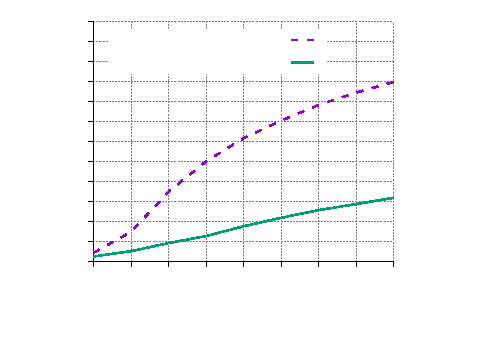
\includegraphics{figures/concat-graph-data.pdf}}%
    \gplfronttext
  \end{picture}%
\endgroup

    \end{subfigure}%
    \hspace{-20pt}
    \begin{subfigure}[t]{0.5\textwidth}
      \centering
      % GNUPLOT: LaTeX picture with Postscript
\begingroup
  \makeatletter
  \providecommand\color[2][]{%
    \GenericError{(gnuplot) \space\space\space\@spaces}{%
      Package color not loaded in conjunction with
      terminal option `colourtext'%
    }{See the gnuplot documentation for explanation.%
    }{Either use 'blacktext' in gnuplot or load the package
      color.sty in LaTeX.}%
    \renewcommand\color[2][]{}%
  }%
  \providecommand\includegraphics[2][]{%
    \GenericError{(gnuplot) \space\space\space\@spaces}{%
      Package graphicx or graphics not loaded%
    }{See the gnuplot documentation for explanation.%
    }{The gnuplot epslatex terminal needs graphicx.sty or graphics.sty.}%
    \renewcommand\includegraphics[2][]{}%
  }%
  \providecommand\rotatebox[2]{#2}%
  \@ifundefined{ifGPcolor}{%
    \newif\ifGPcolor
    \GPcolortrue
  }{}%
  \@ifundefined{ifGPblacktext}{%
    \newif\ifGPblacktext
    \GPblacktexttrue
  }{}%
  % define a \g@addto@macro without @ in the name:
  \let\gplgaddtomacro\g@addto@macro
  % define empty templates for all commands taking text:
  \gdef\gplbacktext{}%
  \gdef\gplfronttext{}%
  \makeatother
  \ifGPblacktext
    % no textcolor at all
    \def\colorrgb#1{}%
    \def\colorgray#1{}%
  \else
    % gray or color?
    \ifGPcolor
      \def\colorrgb#1{\color[rgb]{#1}}%
      \def\colorgray#1{\color[gray]{#1}}%
      \expandafter\def\csname LTw\endcsname{\color{white}}%
      \expandafter\def\csname LTb\endcsname{\color{black}}%
      \expandafter\def\csname LTa\endcsname{\color{black}}%
      \expandafter\def\csname LT0\endcsname{\color[rgb]{1,0,0}}%
      \expandafter\def\csname LT1\endcsname{\color[rgb]{0,1,0}}%
      \expandafter\def\csname LT2\endcsname{\color[rgb]{0,0,1}}%
      \expandafter\def\csname LT3\endcsname{\color[rgb]{1,0,1}}%
      \expandafter\def\csname LT4\endcsname{\color[rgb]{0,1,1}}%
      \expandafter\def\csname LT5\endcsname{\color[rgb]{1,1,0}}%
      \expandafter\def\csname LT6\endcsname{\color[rgb]{0,0,0}}%
      \expandafter\def\csname LT7\endcsname{\color[rgb]{1,0.3,0}}%
      \expandafter\def\csname LT8\endcsname{\color[rgb]{0.5,0.5,0.5}}%
    \else
      % gray
      \def\colorrgb#1{\color{black}}%
      \def\colorgray#1{\color[gray]{#1}}%
      \expandafter\def\csname LTw\endcsname{\color{white}}%
      \expandafter\def\csname LTb\endcsname{\color{black}}%
      \expandafter\def\csname LTa\endcsname{\color{black}}%
      \expandafter\def\csname LT0\endcsname{\color{black}}%
      \expandafter\def\csname LT1\endcsname{\color{black}}%
      \expandafter\def\csname LT2\endcsname{\color{black}}%
      \expandafter\def\csname LT3\endcsname{\color{black}}%
      \expandafter\def\csname LT4\endcsname{\color{black}}%
      \expandafter\def\csname LT5\endcsname{\color{black}}%
      \expandafter\def\csname LT6\endcsname{\color{black}}%
      \expandafter\def\csname LT7\endcsname{\color{black}}%
      \expandafter\def\csname LT8\endcsname{\color{black}}%
    \fi
  \fi
    \setlength{\unitlength}{0.0500bp}%
    \ifx\gptboxheight\undefined%
      \newlength{\gptboxheight}%
      \newlength{\gptboxwidth}%
      \newsavebox{\gptboxtext}%
    \fi%
    \setlength{\fboxrule}{0.5pt}%
    \setlength{\fboxsep}{1pt}%
\begin{picture}(4680.00,3276.00)%
    \gplgaddtomacro\gplbacktext{%
      \csname LTb\endcsname%%
      \put(721,751){\makebox(0,0)[r]{\strut{}$\sfrac{1}{16}$}}%
      \csname LTb\endcsname%%
      \put(721,943){\makebox(0,0)[r]{\strut{}$\sfrac{1}{8}$}}%
      \csname LTb\endcsname%%
      \put(721,1135){\makebox(0,0)[r]{\strut{}$\sfrac{1}{4}$}}%
      \csname LTb\endcsname%%
      \put(721,1327){\makebox(0,0)[r]{\strut{}$\sfrac{1}{2}$}}%
      \csname LTb\endcsname%%
      \put(721,1519){\makebox(0,0)[r]{\strut{}1}}%
      \csname LTb\endcsname%%
      \put(721,1711){\makebox(0,0)[r]{\strut{}2}}%
      \csname LTb\endcsname%%
      \put(721,1903){\makebox(0,0)[r]{\strut{}4}}%
      \csname LTb\endcsname%%
      \put(721,2095){\makebox(0,0)[r]{\strut{}8}}%
      \csname LTb\endcsname%%
      \put(721,2287){\makebox(0,0)[r]{\strut{}16}}%
      \csname LTb\endcsname%%
      \put(721,2479){\makebox(0,0)[r]{\strut{}32}}%
      \csname LTb\endcsname%%
      \put(721,2671){\makebox(0,0)[r]{\strut{}64}}%
      \csname LTb\endcsname%%
      \put(721,2863){\makebox(0,0)[r]{\strut{}128}}%
      \csname LTb\endcsname%%
      \put(721,3055){\makebox(0,0)[r]{\strut{}256}}%
      \csname LTb\endcsname%%
      \put(900,484){\makebox(0,0){\strut{}0}}%
      \csname LTb\endcsname%%
      \put(1260,484){\makebox(0,0){\strut{}}}%
      \csname LTb\endcsname%%
      \put(1620,484){\makebox(0,0){\strut{}100}}%
      \csname LTb\endcsname%%
      \put(1980,484){\makebox(0,0){\strut{}}}%
      \csname LTb\endcsname%%
      \put(2340,484){\makebox(0,0){\strut{}200}}%
      \csname LTb\endcsname%%
      \put(2699,484){\makebox(0,0){\strut{}}}%
      \csname LTb\endcsname%%
      \put(3059,484){\makebox(0,0){\strut{}300}}%
      \csname LTb\endcsname%%
      \put(3419,484){\makebox(0,0){\strut{}}}%
      \csname LTb\endcsname%%
      \put(3779,484){\makebox(0,0){\strut{}400}}%
    }%
    \gplgaddtomacro\gplfronttext{%
      \csname LTb\endcsname%%
      \put(391,1903){\rotatebox{-270}{\makebox(0,0){\strut{}}}}%
      \put(2339,154){\makebox(0,0){\strut{}Number of columns}}%
      \csname LTb\endcsname%%
      \put(3286,1118){\makebox(0,0)[r]{\strut{}implicit join}}%
      \csname LTb\endcsname%%
      \put(3286,898){\makebox(0,0)[r]{\strut{}dependent join}}%
    }%
    \gplbacktext
    \put(0,0){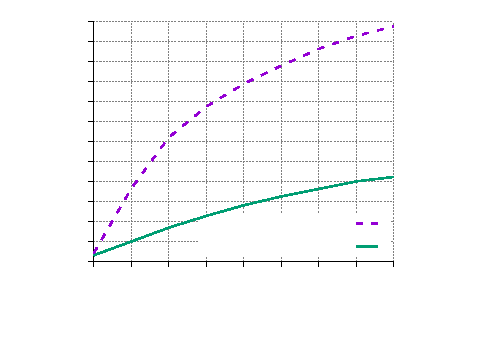
\includegraphics{figures/join-graph-data.pdf}}%
    \gplfronttext
  \end{picture}%
\endgroup

    \end{subfigure}
    \caption{#1}
    \label{fig:dependentVsImplicitBenchmarks}
  \end{figure}
}

\newcommand\timingGraphsZoomedOut[1]{
  \begin{figure}
    \centering
    \begin{subfigure}[t]{0.5\textwidth}
      \centering
      % GNUPLOT: LaTeX picture with Postscript
\begingroup
  \makeatletter
  \providecommand\color[2][]{%
    \GenericError{(gnuplot) \space\space\space\@spaces}{%
      Package color not loaded in conjunction with
      terminal option `colourtext'%
    }{See the gnuplot documentation for explanation.%
    }{Either use 'blacktext' in gnuplot or load the package
      color.sty in LaTeX.}%
    \renewcommand\color[2][]{}%
  }%
  \providecommand\includegraphics[2][]{%
    \GenericError{(gnuplot) \space\space\space\@spaces}{%
      Package graphicx or graphics not loaded%
    }{See the gnuplot documentation for explanation.%
    }{The gnuplot epslatex terminal needs graphicx.sty or graphics.sty.}%
    \renewcommand\includegraphics[2][]{}%
  }%
  \providecommand\rotatebox[2]{#2}%
  \@ifundefined{ifGPcolor}{%
    \newif\ifGPcolor
    \GPcolorfalse
  }{}%
  \@ifundefined{ifGPblacktext}{%
    \newif\ifGPblacktext
    \GPblacktexttrue
  }{}%
  % define a \g@addto@macro without @ in the name:
  \let\gplgaddtomacro\g@addto@macro
  % define empty templates for all commands taking text:
  \gdef\gplbacktext{}%
  \gdef\gplfronttext{}%
  \makeatother
  \ifGPblacktext
    % no textcolor at all
    \def\colorrgb#1{}%
    \def\colorgray#1{}%
  \else
    % gray or color?
    \ifGPcolor
      \def\colorrgb#1{\color[rgb]{#1}}%
      \def\colorgray#1{\color[gray]{#1}}%
      \expandafter\def\csname LTw\endcsname{\color{white}}%
      \expandafter\def\csname LTb\endcsname{\color{black}}%
      \expandafter\def\csname LTa\endcsname{\color{black}}%
      \expandafter\def\csname LT0\endcsname{\color[rgb]{1,0,0}}%
      \expandafter\def\csname LT1\endcsname{\color[rgb]{0,1,0}}%
      \expandafter\def\csname LT2\endcsname{\color[rgb]{0,0,1}}%
      \expandafter\def\csname LT3\endcsname{\color[rgb]{1,0,1}}%
      \expandafter\def\csname LT4\endcsname{\color[rgb]{0,1,1}}%
      \expandafter\def\csname LT5\endcsname{\color[rgb]{1,1,0}}%
      \expandafter\def\csname LT6\endcsname{\color[rgb]{0,0,0}}%
      \expandafter\def\csname LT7\endcsname{\color[rgb]{1,0.3,0}}%
      \expandafter\def\csname LT8\endcsname{\color[rgb]{0.5,0.5,0.5}}%
    \else
      % gray
      \def\colorrgb#1{\color{black}}%
      \def\colorgray#1{\color[gray]{#1}}%
      \expandafter\def\csname LTw\endcsname{\color{white}}%
      \expandafter\def\csname LTb\endcsname{\color{black}}%
      \expandafter\def\csname LTa\endcsname{\color{black}}%
      \expandafter\def\csname LT0\endcsname{\color{black}}%
      \expandafter\def\csname LT1\endcsname{\color{black}}%
      \expandafter\def\csname LT2\endcsname{\color{black}}%
      \expandafter\def\csname LT3\endcsname{\color{black}}%
      \expandafter\def\csname LT4\endcsname{\color{black}}%
      \expandafter\def\csname LT5\endcsname{\color{black}}%
      \expandafter\def\csname LT6\endcsname{\color{black}}%
      \expandafter\def\csname LT7\endcsname{\color{black}}%
      \expandafter\def\csname LT8\endcsname{\color{black}}%
    \fi
  \fi
    \setlength{\unitlength}{0.0500bp}%
    \ifx\gptboxheight\undefined%
      \newlength{\gptboxheight}%
      \newlength{\gptboxwidth}%
      \newsavebox{\gptboxtext}%
    \fi%
    \setlength{\fboxrule}{0.5pt}%
    \setlength{\fboxsep}{1pt}%
\begin{picture}(4680.00,3276.00)%
    \gplgaddtomacro\gplbacktext{%
      \csname LTb\endcsname%%
      \put(296,751){\makebox(0,0)[r]{\strut{}$0$}}%
      \csname LTb\endcsname%%
      \put(296,981){\makebox(0,0)[r]{\strut{}$2$}}%
      \csname LTb\endcsname%%
      \put(296,1212){\makebox(0,0)[r]{\strut{}$4$}}%
      \csname LTb\endcsname%%
      \put(296,1442){\makebox(0,0)[r]{\strut{}$6$}}%
      \csname LTb\endcsname%%
      \put(296,1673){\makebox(0,0)[r]{\strut{}$8$}}%
      \csname LTb\endcsname%%
      \put(296,1903){\makebox(0,0)[r]{\strut{}$10$}}%
      \csname LTb\endcsname%%
      \put(296,2133){\makebox(0,0)[r]{\strut{}$12$}}%
      \csname LTb\endcsname%%
      \put(296,2364){\makebox(0,0)[r]{\strut{}$14$}}%
      \csname LTb\endcsname%%
      \put(296,2594){\makebox(0,0)[r]{\strut{}$16$}}%
      \csname LTb\endcsname%%
      \put(296,2825){\makebox(0,0)[r]{\strut{}$18$}}%
      \csname LTb\endcsname%%
      \put(296,3055){\makebox(0,0)[r]{\strut{}$20$}}%
      \csname LTb\endcsname%%
      \put(475,484){\makebox(0,0){\strut{}0}}%
      \csname LTb\endcsname%%
      \put(848,484){\makebox(0,0){\strut{}}}%
      \csname LTb\endcsname%%
      \put(1221,484){\makebox(0,0){\strut{}50}}%
      \csname LTb\endcsname%%
      \put(1594,484){\makebox(0,0){\strut{}}}%
      \csname LTb\endcsname%%
      \put(1967,484){\makebox(0,0){\strut{}100}}%
      \csname LTb\endcsname%%
      \put(2340,484){\makebox(0,0){\strut{}}}%
      \csname LTb\endcsname%%
      \put(2712,484){\makebox(0,0){\strut{}150}}%
      \csname LTb\endcsname%%
      \put(3085,484){\makebox(0,0){\strut{}}}%
      \csname LTb\endcsname%%
      \put(3458,484){\makebox(0,0){\strut{}200}}%
      \csname LTb\endcsname%%
      \put(3831,484){\makebox(0,0){\strut{}}}%
      \csname LTb\endcsname%%
      \put(4204,484){\makebox(0,0){\strut{}250}}%
    }%
    \gplgaddtomacro\gplfronttext{%
      \csname LTb\endcsname%%
      \put(-188,1903){\rotatebox{-270}{\makebox(0,0){\strut{}Compilation time (seconds)}}}%
      \put(2339,154){\makebox(0,0){\strut{}List size}}%
      \csname LTb\endcsname%%
      \put(1861,2882){\makebox(0,0)[r]{\strut{}Implicits}}%
      \csname LTb\endcsname%%
      \put(1861,2662){\makebox(0,0)[r]{\strut{}Singletons}}%
      \csname LTb\endcsname%%
      \put(1861,2442){\makebox(0,0)[r]{\strut{}Match Types}}%
    }%
    \gplbacktext
    \put(0,0){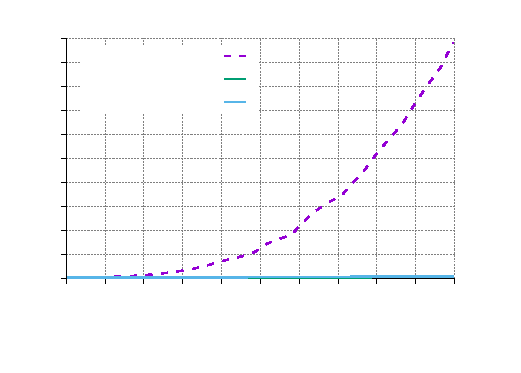
\includegraphics{figures/concat}}%
    \gplfronttext
  \end{picture}%
\endgroup

    \end{subfigure}%
    \hspace{-20pt}
    \begin{subfigure}[t]{0.5\textwidth}
      \centering
      \input{figures/remove.gex}
    \end{subfigure}

    \vspace{-2pt}
    \begin{subfigure}[t]{0.5\textwidth}
      \centering
      \input{figures/join.gex}
    \end{subfigure}%
    \hspace{-20pt}
    \begin{subfigure}[t]{0.5\textwidth}
      \centering
      \input{figures/reduce.gex}
    \end{subfigure}
    \caption{#1}
    \label{fig:timingGraphsZoomedOut}
  \end{figure}
}

\newcommand\timingGraphsZoomedIn[1]{
  \begin{figure}[!ht]
    \centering
    \begin{subfigure}[t]{0.5\textwidth}
      \centering
      \input{figures/concat-2.gex}
    \end{subfigure}%
    \hspace{-20pt}
    \begin{subfigure}[t]{0.5\textwidth}
      \centering
      \input{figures/remove-2.gex}
    \end{subfigure}

    \vspace{-2pt}
    \begin{subfigure}[t]{0.5\textwidth}
      \centering
      \input{figures/join-2.gex}
    \end{subfigure}%
    \hspace{-20pt}
    \begin{subfigure}[t]{0.5\textwidth}
      \centering
      \input{figures/reduce-2.gex}
    \end{subfigure}
    \caption{#1}
    \label{fig:timingGraphsZoomedIn}
  \end{figure}
}

\newcommand\timingGraphsTooEarlyTooLate[1]{
  \begin{figure}
    \centering
    \begin{subfigure}[t]{0.5\textwidth}
      \centering
      \input{figures/2early2late.gex}
    \end{subfigure}%
    \caption{#1}
    \label{fig:timingGraphsTooEarlyTooLate}
  \end{figure}
}

\newcommand\bytecodeSizeTable[1]{
  \begin{table*}
    \centering
    \caption{#1}
    \label{fig:bytecodeSizeTable}
    \renewcommand{\arraystretch}{1.2}
    \begin{tabular}{@{}lrrr@{}}
    \toprule & Implicits & Singletons & Match Types \\
    \midrule
    Concat & 6  & 0 & 0 \\
    Remove & 6  & 0 & 0 \\
    Reduce & 12 & 0 & 0 \\
    Join   & 18 & 0 & 0 \\
    \bottomrule
    \end{tabular}
  \end{table*}
}

\newcommand\regexBars[1]{
  \begin{figure}
    \centering
    \hspace{-15pt}
    \begin{subfigure}[t]{0.5\textwidth}
      \centering
      \input{figures/regex-compiletime.gex}
    \end{subfigure}%
    \hspace{10pt}
    \begin{subfigure}[t]{0.5\textwidth}
      \centering
      \input{figures/regex-runtime.gex}
    \end{subfigure}
    \caption{#1}
    \label{fig:regexBars}
  \end{figure}
}
